\section{График функции}
\textbf{Преобразование графиков ф-ий:}

\begin{enumerate}
	
	\item \textbf{Симметрия относительно осей координат}
	\begin{itemize}
		\item 
		Функции $y = f(x)$ и $y = -f(x)$ имеют одну и ту же область определения, их графики симметричны относительно оси $Ox$.
		%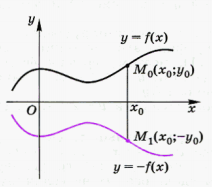
\includegraphics[scale=1]{./mh/math_analysis/functions/graph1.png}\\
		\item 
		Функции $y = f(x)$ и $y = f(-x)$ имеют области определения, симметричные относительно точки $O$. Их графики симметричны относительно оси $Oy$.
		%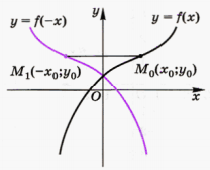
\includegraphics[scale=1]{./mh/math_analysis/functions/graph2.png}\\
	\end{itemize}

	\item \textbf{Сдвиг вдоль осей координат (параллельный перенос)}
	\begin{itemize}
		\item 
		Функция $y = f(x - a)$, где $a \neq 0$, определена для всех $x$, таких, что $(x - a) \in D(f(x))$. График ф-ии $y = f(x - a)$ 
		получается сдвигом вдоль оси $Ox$ на величину $|a|$ графика функции $y = f(x)$ вправо, если $a > 0$, 
		и влево, если $a < 0$.
		\item
		Функция $y = f(x) + B$, где $B \neq 0$, имеет ту же область определения, что и ф-ия $y = f(x)$. График ф-ии $y = f(x) + B$ 
		получается сдвигом вдоль оси $Oy$ на величину $|B|$ графика функции $y = f(x)$ вверх, если $B > 0$, 
		и вниз, если $B < 0$.
	\end{itemize}
	
	\item \textbf{Растяжение с сжатие графика вдоль всей оси координат}\\
	
	\item \textbf{Построение графика функции $y = Af(k(x - a)) + B)$ по графику функции $y = f(x)$}\\
	
	\item \textbf{Симметрия относительно прямой $y = x$}\\
	
\end{enumerate}

